\documentclass[a4paper, 7pt, landscape]{scrartcl}
\usepackage[german]{babel}
\usepackage[utf8]{inputenc}
\usepackage{multicol}
\usepackage{geometry}
\usepackage{graphicx}
\usepackage{wrapfig}
\usepackage{enumitem}
\usepackage{fancyhdr}
\usepackage{index}
\usepackage{sectsty}
\usepackage{mwe}
\usepackage{comment}
\usepackage{lipsum}
\usepackage{titlesec}
\usepackage[dvipsnames]{xcolor}
\usepackage{amsmath}
\usepackage{amssymb}
\usepackage{listings}

%Define Math Commands:
\newcommand*{\field}[1]{\mathbb{#1}}%
\newcommand{\Mod}[1]{\ (\mathrm{mod}\ #1)}

%Image Folder:
\graphicspath{{../img/}}

%format
\geometry{top=0.4cm,left=0.5cm,right=0.5cm,bottom=0.4cm}
\setlist{topsep=0pt, leftmargin=5mm, nolistsep}

% Code Snippets

\definecolor{javared}{rgb}{0.6,0,0} % for strings

\lstset{
language=C,
basicstyle=\fontsize{7}{7} \ttfamily,
keywordstyle=\bfseries\color{RoyalBlue},
stringstyle=\color{javared},
commentstyle=\color{MidnightBlue},
morecomment=[s][\color{MidnightBlue}]{/**}{*/},
tabsize=2,
showspaces=false,
showstringspaces=false,
texcl = true,
rulecolor = \color{black},
breaklines = true,
aboveskip = 0em,
belowskip = 0em
}




% Define Section Format
\titleformat{name=\section}[block]
{\sffamily\normalsize}
{}
{0pt}
{\colorsection}
\titlespacing*{\section}{0pt}{0pt}{0pt}

\newcommand{\colorsection}[1]{%
\colorbox{MidnightBlue!40}{\parbox{0.98\linewidth}{\color{black}\thesection\ #1}}}


% Define Subsection Format
\titleformat{name=\subsection}[block]
{\sffamily\small}
{}
{0pt}
{\colorsubsection}
\titlespacing*{\subsection}{0pt}{0pt}{0pt}

\newcommand{\colorsubsection}[1]{%
\colorbox{YellowGreen!50}{\parbox{0.98\linewidth}{\color{black}\thesubsection\ #1}}}

% Define SubSubsection Format
\titleformat{name=\subsubsection}[block]
{\sffamily\small}
{}
{0pt}
{\colorsubsubsection}
\titlespacing*{\subsubsection}{0pt}{0pt}{0pt}

\newcommand{\colorsubsubsection}[1]{%
\colorbox{Goldenrod!50}{\parbox{0.98\linewidth}{\color{black}\thesubsubsection\ #1}}}

% -----------------------------------------------------------------------
\begin{document}
    %	\pagecolor{p}
    %	\color{t}
    \setlength{\columnseprule}{0.4pt}
    \footnotesize
    \begin{multicols*}{2}

        %! Author = Philipp Emmenegger
%! Date = 30/06/2021

\section{Einführung}
\textbf{Nutzen ComBau}
\begin{itemize}
    \item Programmiersprachen und Sprachkonzepte besser verstehen
    \item Sprachfeatures beurteilen können
    \item Konzepte in verwandten Bereichen einsetzen
\end{itemize}

\subsection{Begriffe}
\textbf{Compiler}
\begin{itemize}
    \item Transformiert Quellcode in Maschinencode
\end{itemize}
\textbf{Runtime System}
\begin{itemize}
    \item Unterstützt die Programmausführung mit Software und Hardware Mechanismen
\end{itemize}
\textbf{Syntax}
\begin{itemize}
    \item Definiert Struktur des Programms
    \item Bewährte Formalismen für Syntax
\end{itemize}
\textbf{Semantik}
\begin{itemize}
    \item Definiert Bedeutung des Programms
    \item Meist in Prosa beschrieben
\end{itemize}

\subsection{Architekturen}
\begin{center}
    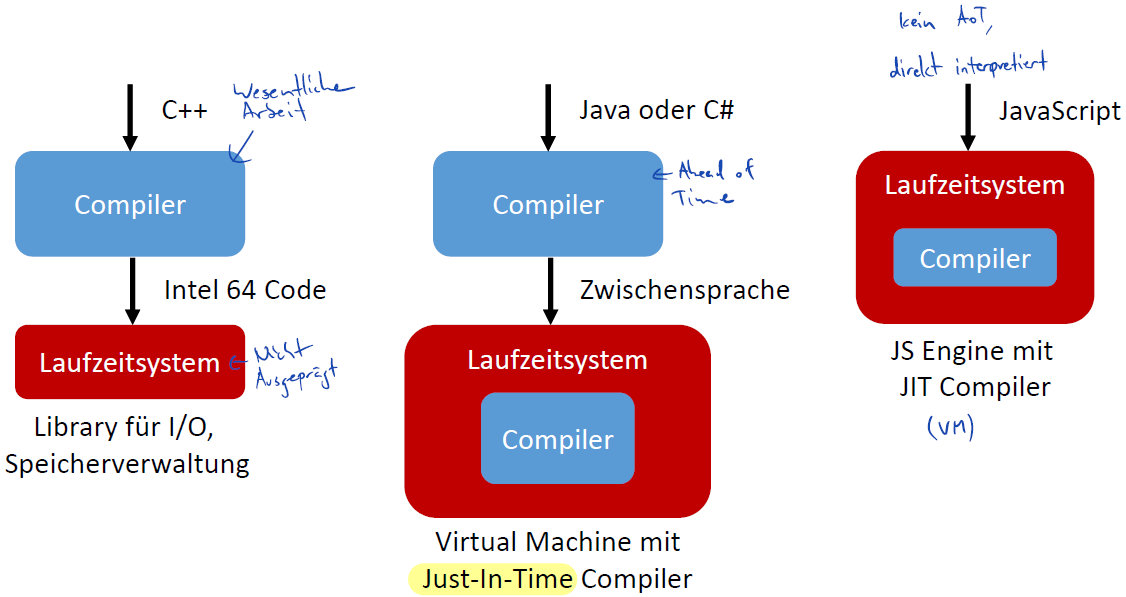
\includegraphics[width=0.6\linewidth]{/architekturen.png} 
\end{center}

\subsection{Aufbau Compiler}
\begin{center}
    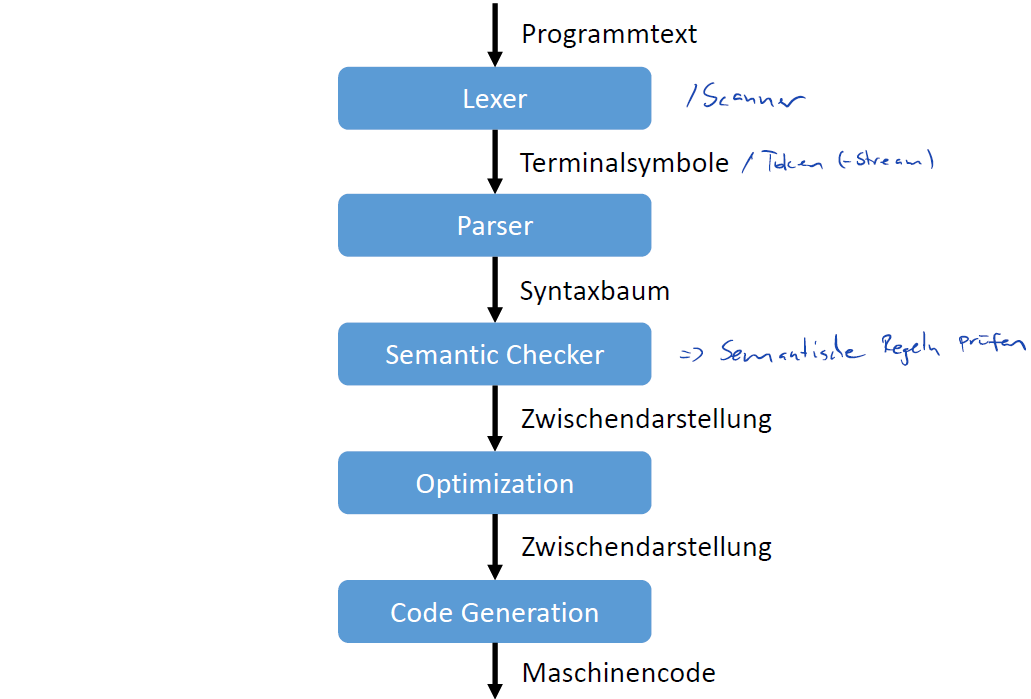
\includegraphics[width=0.5\linewidth]{/aufbau_compiler.png} 
\end{center}
\subsubsection{Lexer}
\textbf{Lexikalische Analyse, Scanner}
\begin{itemize}
    \item Zerlegt Programmtext in Terminalsymbole (Tokens)
    \item keine Tiefenstruktur
\end{itemize}
\subsubsection{Parser}
\textbf{Syntaktische Analyse}
\begin{itemize}
    \item Erzeugt Syntaxbaum gemäss Programmstruktur
    \item Kontextfreie Sprache
\end{itemize}
\subsubsection{Semantic Checker}
\textbf{Semantische Analyse}
\begin{itemize}
    \item Löst Symbole auf
    \item Prüft Typen und semantische Regeln
\end{itemize}
\subsubsection{Optimization}
\begin{itemize}
    \item Wandelt Zwischendarstellung in effizientere um
\end{itemize}
\subsubsection{Code Generation}
\begin{itemize}
    \item Erzeugt ausführbarer Maschinencode
\end{itemize}
\subsubsection{Zwischenarstellung}
\textbf{Intermediate Representation}
\begin{itemize}
    \item Beschreibt Programm als Datenstruktur (diverse Varianten)
\end{itemize}

\subsection{Aufbau Laufzeitsystem}
\begin{center}
    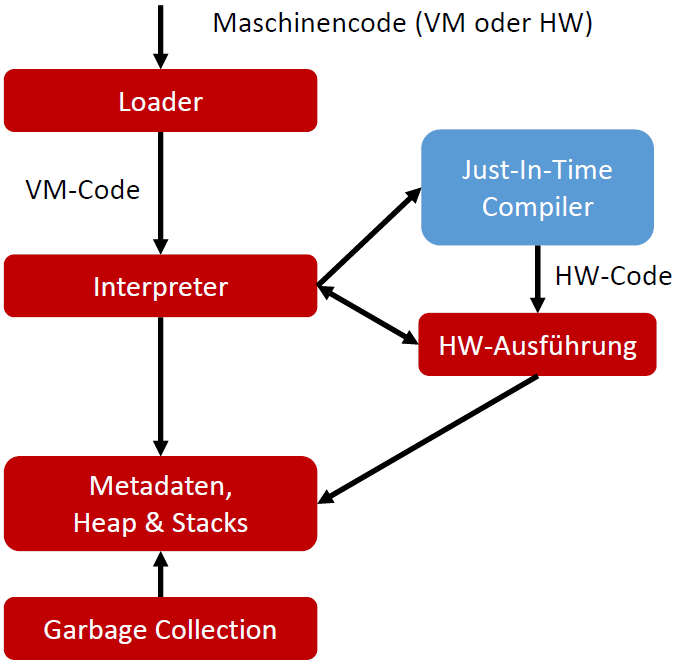
\includegraphics[width=0.4\linewidth]{/aufbau_laufzeitsystem.png} 
\end{center}
\subsubsection{Loader}
\begin{itemize}
    \item Lädt Maschinencode in Speicher
    \item Veranlasst Ausführung
\end{itemize}
\subsubsection{Interpreter}
\begin{itemize}
    \item Liest Instruktionen und emuliert diese in Software
\end{itemize}
\subsubsection{JIT (Just-In-Time) Compiler}
\begin{itemize}
    \item Übersetzt Code-Teile in Hardware-Instruktionscode
\end{itemize}
\subsubsection{HW-Ausführung (nativ)}
\begin{itemize}
    \item Lässt Instruktionscode direkt auf HW-Prozessor laufen
\end{itemize}
\subsubsection{Metadaten, Heap + Stacks}
\begin{itemize}
    \item Merken Programminfos, Objekte und Prozeduraufrufe
\end{itemize}
\subsubsection{Garbage Collection}
\begin{itemize}
    \item Räumt nicht erreichbare Objecte ab
\end{itemize}
\newpage

\subsection{Syntax}
\subsubsection{EBNF}
\textbf{Extended Backus-Naur Form}
\begin{center}
    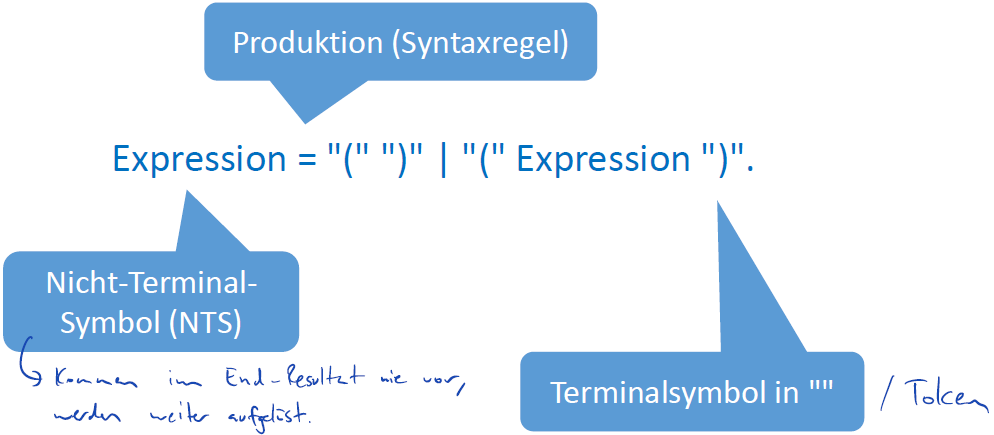
\includegraphics[width=0.5\linewidth]{/ebnf.png} 
    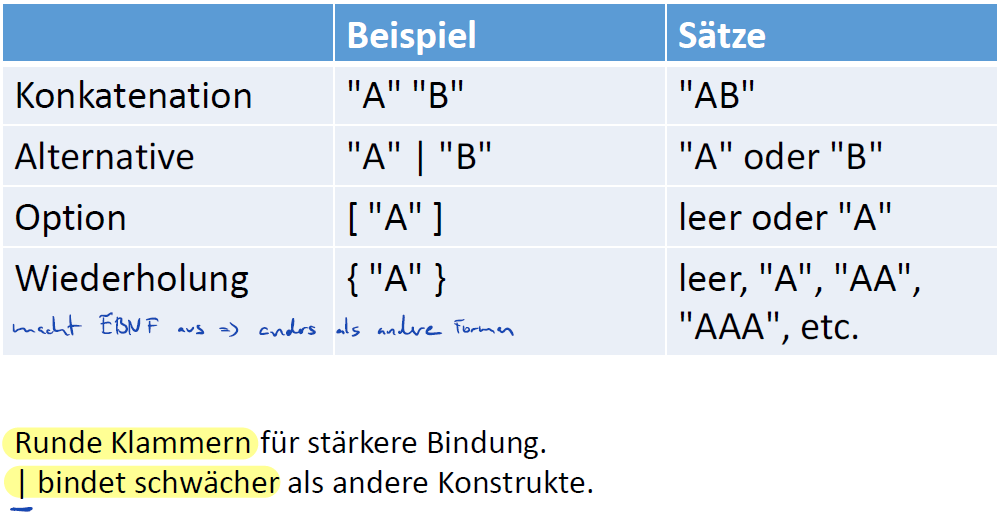
\includegraphics[width=0.5\linewidth]{/ebnf_regeln.png} 
\end{center}
\subsubsection{Arithmetische Ausdrücke}
\begin{center}
    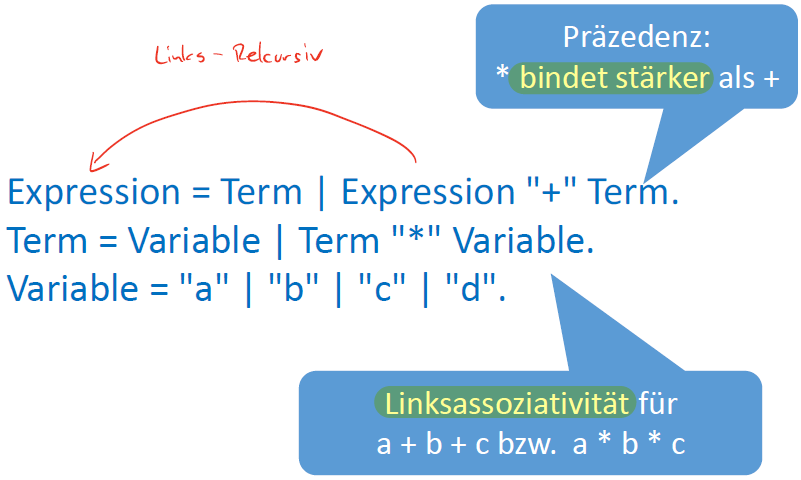
\includegraphics[width=0.5\linewidth]{/ebnf_arithmetisch.png} 
\end{center}

    \end{multicols*}
\end{document}

























